\subsubsection{Rauheit}
Die Rauheit der Graphitschicht konnte mit der Software f�r das RTM bestimmt werden, nachdem die Graphitschicht im CC-Modus mit der Spitze des RTM abgerastert wurde. Die Verkippung wurde bestimmt und grob bis auf \SI{0,2}{\degree} korrigiert. Das Fenster Topography-Scan ist f�r die Messung nicht wichtig, da es die Oberfl�chenbeschaffenheit ausschlie�lich auf H�he des schwarzen Pfeils angibt. In Abbildung \ref{fig:lin_rau_graph} ist die Messung zur Bestimmung der mittleren Linienrauheit dargestellt.
\begin{figure}[H]
\centering
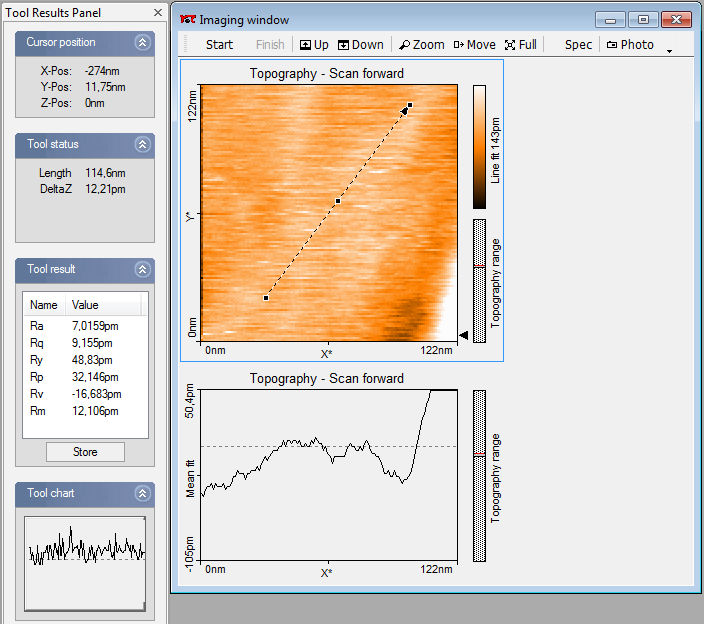
\includegraphics[scale = 0.75]{snipping_122_linienrauheit}
\caption{ Mittlere Linienrauheit von Graphit entlang der abgebildeten Linie \\ ($R_a = \SI{7,0159}{pm}$ und $R_q = \SI{9,1550}{pm}$) }
\label{fig:lin_rau_graph}
\end{figure}
Ebenso wurde die mittlere Fl�chenrauheit der Graphitprobe bestimmt, welche in Abbildung \ref{fig:flae_rau_graph} dargestellt ist.
\begin{figure}[H]
\centering
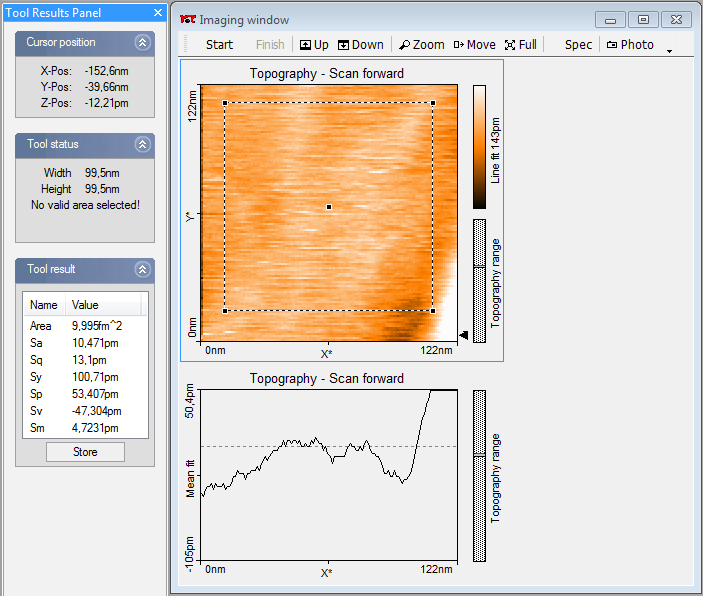
\includegraphics[scale = 0.75]{snipping_122_flaechenrauheit}
\caption{ Mittlere Fl�chenrauheit von Graphit f�r die Fl�che im Quadrat \\ ($S_a = \SI{10,471}{pm}$ und $S_q = \SI{13,100}{pm}$) }
\label{fig:flae_rau_graph}
\end{figure}
Man sieht, dass die mittlere Fl�chenrauheit gr��er als die mittlere Linienrauheit ist, wobei der Anteil der arithmetischen Rauheit an der quadratischen Rauheit bei beiden Messungen in etwa gleich gro� ist ($\frac{R_a}{R_q} = 0,78 = 78 \%$ und $\frac{S_a}{S_q} = 0,80 = 80 \%$). F�r die Linienrauheit wurde eine m�glichst glatte Linie gew�hlt, wodurch der Unterschied zur quadratischen Rauheit begr�ndet werden kann. Insgesammt f�llt auf, dass die Oberfl�chenrauheit von HOP-Graphit relativ gering ist. Die �hnlchkeit von Linienrauheit und Fl�chenrauheit sprechen bei dieser Oberfl�che f�r eine gute Messung. 